
%%%%%%%%%%%%%%%%%%%%%%%%%%%%%%%%%%%%%%%%%%%%%%%%%%%%%%%%%%%%%%%%%%%%%%%%%%%%%%%%
\section{Services}
%%%%%%%%%%%%%%%%%%%%%%%%%%%%%%%%%%%%%%%%%%%%%%%%%%%%%%%%%%%%%%%%%%%%%%%%%%%%%%%%
\begin{frame}
\frametitle{Services}
\begin{itemize}
\item A \alert{service} is simply a piece of code that runs in the background of your application. It doesn’t have a user interface
\item The only states for ``bound'' services are started and stopped (destroyed)
\item The Yamba application needs to create a service to periodically
connect to the cloud and check for new statuses from the user’s friends. This
service will be always on and always running, regardless of whether the user ever starts
\end{itemize}
\end{frame}
%------------------------------------------------------------------------------
\subsection{The Yamba Application Object}
%%%%%%%%%%%%%%%%%%%%%%%%%%%%%%%%%%%%%%%%%%%%%%%%%%%%%%%%%%%%%%%%%%%%%%%%%%%%%%%%
\begin{frame}
\frametitle{The Yamba Application Object}
An \texttt{Application} object represents the common state of your entire application.
We are going to create our own instance of this object and call it \texttt{YambaApplication}. The
steps for creating the \texttt{YambaApplication} class are:
\begin{enumerate}
\item Create the Java class representing \texttt{YambaApplication}
\item Register the new class with the \texttt{AndroidManifest.xml} file
\end{enumerate}
\end{frame}
%------------------------------------------------------------------------------
\begin{frame}[containsverbatim]
\frametitle{The Yamba Application Class}
Create a new Java class in the same package as the rest of our
classes. Call this class \texttt{YambaApplication}, and it will extend the \texttt{Application} base
class from the framework
\lstset{language=java, style=eclipse, breaklines=true, tabsize=2}
\begin{adjustbox}{width=1.0 \textwidth}
\begin{lstlisting}[caption=src/com/artemisa/yamba/YambaApplication.java, basicstyle=\tiny,escapechar=!]
package com/artemisa/yamba;

import android.app.Application;

public class YambaApplication extends Application { // !\circled{1}!

}
\end{lstlisting}
\end{adjustbox}
\end{frame}
%------------------------------------------------------------------------------
\begin{frame}[allowframebreaks,containsverbatim]
\frametitle{\texttt{YambaApplication.java}}
Move common tasks into this base object

\lstset{language=java, style=eclipse, breaklines=true, tabsize=2}
\begin{lstlisting}[caption=src/com/artemisa/yamba/YambaApplication.java, basicstyle=\tiny,escapechar=!]
// .
// .
// .
public class YambaApplication extends Application implements
		OnSharedPreferenceChangeListener { // !\circled{1}!
	private static final String TAG = YambaApplication.class.getSimpleName();
	private Twitter twitter; // !\circled{2}!
	private SharedPreferences prefs;

	@Override
	public void onCreate() { // !\circled{3}!
		// TODO Auto-generated method stub
		super.onCreate();
		prefs = PreferenceManager.getDefaultSharedPreferences(this);
		prefs.registerOnSharedPreferenceChangeListener(this);
		Log.i(TAG, "onCreated");
	}

	@Override
	public void onTerminate() { // !\circled{4}!
		// TODO Auto-generated method stub
		super.onTerminate();
		Log.i(TAG, "onTerminated");
	}

	public synchronized Twitter getTwitter() { // !\circled{5}!
		if (twitter == null) {
			String username, password, apiRoot;
			username = prefs.getString("username", "");
			password = prefs.getString("password", "");
			apiRoot = prefs.getString("apiRoot",
					"http://yamba.marakana.com/api");
			// Connect to twitter.com
			twitter = new Twitter(username, password);
			twitter.setAPIRootUrl(apiRoot);
		}
		return twitter;
	}

	@Override
	public synchronized void onSharedPreferenceChanged(
			SharedPreferences sharedPreferences, String key) { // !\circled{6}!
		// TODO Auto-generated method stub
		Log.d(TAG, "onSharedPreferenceChanged()");
		twitter = null;

	}
}
\end{lstlisting}
\end{frame}
%------------------------------------------------------------------------------
\begin{frame}[containsverbatim]
\frametitle{Update de Manifest File \texttt{AndroidManifest.xml}}
\centering
\includegraphics[width= 0.75 \textwidth]{update-manifest.eps}
\end{frame}
%------------------------------------------------------------------------------
\begin{frame}[allowframebreaks,containsverbatim]
\frametitle{\texttt{AndroidManifest.xml}}
\lstset{language=XML, style=eclipse,breaklines=true,  basicstyle=\tiny,tabsize=2}
\begin{lstlisting}[caption=AndroidManifest.xml, basicstyle=\tiny,escapechar=$]
<?xml version="1.0" encoding="utf-8"?>
    <!-- . -->
    <!-- . -->
    <!-- . -->

    <application
        android:name="YambaApplication" $\circled{1}$
        android:allowBackup="true"
        android:icon="@drawable/ic_launcher"
        android:label="@string/app_name"
        android:theme="@style/AppTheme" >
        <!-- . -->
        <!-- . -->
        <!-- . -->
    </application>

</manifest>
\end{lstlisting}
\end{frame}
%------------------------------------------------------------------------------
\begin{frame}[allowframebreaks,containsverbatim]
\frametitle{The StatusActivity Java Class}
\lstset{language=java, style=eclipse, breaklines=true, tabsize=2}
%\begin{adjustbox}{width=1.0 \textwidth}
\centering
\begin{lstlisting}[caption=src/com/artemisa/yamba/StatusActivity.java, basicstyle=\tiny,, escapechar=! ]
// .
// .
// .
public class StatusActivity extends Activity implements OnClickListener,
		TextWatcher { \\ !\circled{1}!

	// .
	// .
	// .

	private class PostToTwitter extends AsyncTask<String, Integer, String> {
		@Override
		protected String doInBackground(String... params) {
			// TODO Auto-generated method stub
			try {
				Twitter.Status status = ((YambaApplication) getApplication()).getTwitter().setStatus(params[0]); // !\circled{2}!
				return status.text;

			} catch (TwitterException e) {
				Log.e(TAG, e.toString());
				e.printStackTrace();
				return "Failed to post";
			}
		}

		// .
		// .
		// .
	}
	// .
	// .
	// .
	
}

\end{lstlisting}
%\end{adjustbox}
\end{frame}
%------------------------------------------------------------------------------
\begin{frame}[fragile]
\frametitle{Git}
\begin{enumerate}
\item \texttt{git status}
\item \texttt{git add .}
\item \texttt{git status}
\item \texttt{git commit -a -m ``Yamba Application Object''}
\end{enumerate}

\end{frame}
%------------------------------------------------------------------------------
\subsection{Updater Service}
\begin{frame}
\frametitle{Updater Service}
Steps to creating a service are:
\begin{enumerate}
\item Create the Java class representing your service
\item Register the service in the Android manifest file
\item Start the service
\end{enumerate}
\end{frame}
%------------------------------------------------------------------------------
\begin{frame}
\frametitle{Create the Java class \texttt{UpdaterService.java}}
The basic procedure for creating a service, as with activities and other main building
blocks, is to subclass a \texttt{Service} class provided by the Android framework
\begin{columns}
\column{0.45 \textwidth}
\begin{itemize}
\item \texttt{onCreate()} Called when the service is created for the first time
\item \texttt{onStartCommand()} Called when the service is started
\item \texttt{onDestroy()} Called when the service is terminated
\end{itemize}
\column{0.55 \textwidth}
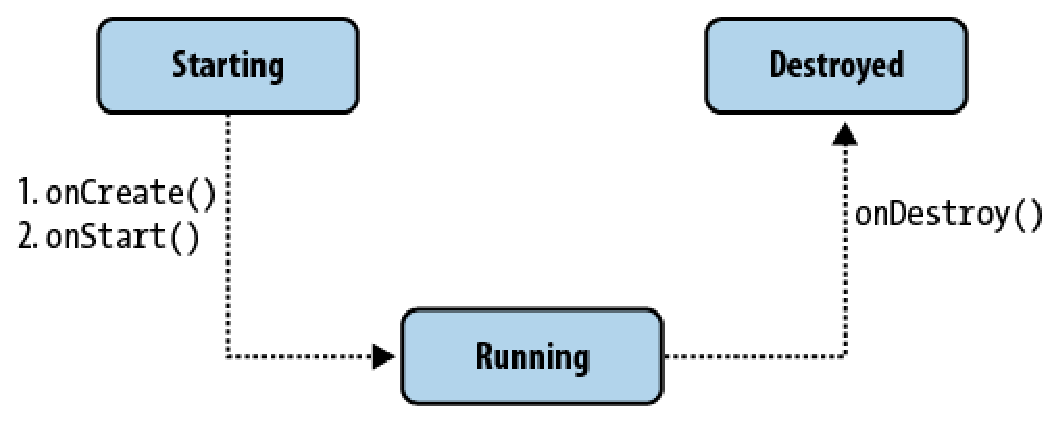
\includegraphics[width= 1.10 \textwidth]{fig-078.eps}
\end{columns}
\end{frame}
%------------------------------------------------------------------------------
\begin{frame}[allowframebreaks,containsverbatim]
\frametitle{\texttt{UpdaterService.java}}
Create the Java class representing \texttt{UpdaterService}

\lstset{language=java, style=eclipse, breaklines=true, tabsize=2}
\begin{lstlisting}[caption=src/com/artemisa/yamba/UpdaterService.java, basicstyle=\tiny,escapechar=!]
// .
// .
// .
public class UpdaterService extends Service {
	static final String TAG = "UpdaterService"; // !\circled{1}!

	@Override
	public IBinder onBind(Intent arg0) { !\circled{2}!
		// TODO Auto-generated method stub
		return null;
	}

	@Override
	public void onCreate() {  // !\circled{3}!
		// TODO Auto-generated method stub
		super.onCreate();
		Log.d(TAG, "onCreated");
	}

	@Override
	public void onDestroy() {  !\circled{4}!
		// TODO Auto-generated method stub
		super.onDestroy();
		Log.d(TAG, "onDestroyed");
	}

	@Override
	public int onStartCommand(Intent intent, int flags, int startId) { !\circled{5}!
		// TODO Auto-generated method stub
		super.onStartCommand(intent, flags, startId);
		Log.d(TAG, "onStarted");
		return START_STICKY;
	}

}
\end{lstlisting}
\end{frame}
%------------------------------------------------------------------------------
\begin{frame}[allowframebreaks,containsverbatim]
\frametitle{Update de Manifest File \texttt{AndroidManifest.xml}}
\lstset{language=XML, style=eclipse,breaklines=true, tabsize=2}
\begin{lstlisting}[caption=AndroidManifest.xml, basicstyle=\tiny,escapechar=$]
<?xml version="1.0" encoding="utf-8"?>
<manifest xmlns:android="http://schemas.android.com/apk/res/android"
    <!-- . -->
    <!-- . -->
    <!-- . -->

        <service android:name="com/artemisa/yamba.UpdaterService" > <!-- $\circled{1}$ -->
        </service>
    </application>

</manifest>
\end{lstlisting}
\end{frame}
%------------------------------------------------------------------------------
\begin{frame}[allowframebreaks,containsverbatim]
\frametitle{Add Menu Items}
We need a way to start and stop the service.
The easiest way would be to add a menu button to our options menu 
\lstset{language=XML, style=eclipse,breaklines=true, tabsize=2}
\begin{lstlisting}[caption=res/menu/status.xml, basicstyle=\tiny,escapechar=$]
<menu xmlns:android="http://schemas.android.com/apk/res/android" >

    <!-- . -->
    <!-- . -->
    <!-- . -->
    <item <!- $\circled{1}$ -->
        android:id="@+id/itemServiceStart"
        android:icon="@android:drawable/ic_media_play"
        android:title="@string/tittleServiceStart">
    </item>
    <item <!- $\circled{2}$ -->
        android:id="@+id/itemServiceStop"
        android:icon="@android:drawable/ic_media_pause"
        android:title="@string/tittleServiceStop">
    </item>

</menu>
\end{lstlisting}
\end{frame}
%------------------------------------------------------------------------------
\begin{frame}[allowframebreaks,containsverbatim]
\frametitle{Update the Options Menu Handling}
\lstset{language=java, style=eclipse, breaklines=true, tabsize=2}
\begin{lstlisting}[caption=src/com/artemisa/yamba/StatusActiviy.java, basicstyle=\tiny,escapechar=!]
// .
// .
// .
// Called when an options item is clicked
@Override
public boolean onOptionsItemSelected(MenuItem item) {
	switch (item.getItemId()) {
	case R.id.itemServiceStart:
		startService(new Intent(this, UpdaterService.class)); // !\circled{1}!
		break;
	case R.id.itemServiceStop:
		stopService(new Intent(this, UpdaterService.class)); //  !\circled{2}!
		break;
	case R.id.itemPrefs:
		startActivity(new Intent(this, PrefsActivity.class));
		break;
	}
	return true;
}
\end{lstlisting}
\end{frame}

%------------------------------------------------------------------------------
\begin{frame}[allowframebreaks,containsverbatim]
\frametitle{Testing the Serivce}
To verify that your service is working
\begin{itemize}
 \item  Open up your LogCat and look for the appropriate
log messages that you generated in your service code
 \item Or press \texttt{Menu} and choose \texttt{Setting|Application|Running services}
\end{itemize}

\end{frame}
%------------------------------------------------------------------------------
\begin{frame}[fragile]
\frametitle{Git}
\begin{enumerate}
\item \texttt{git status}
\item \texttt{git add .}
\item \texttt{git status}
\item \texttt{git commit -a -m ``UpdaterStatus''}
\end{enumerate}

\end{frame}
%------------------------------------------------------------------------------
\begin{frame}[allowframebreaks,containsverbatim]
\frametitle{Looping in the Service}
\begin{itemize}
\item Our service is supposed to wake up every so often, check the online service
for new status updates, an then go back to ``sleep'' for some time
\item A  way to implement this is to have our service run in a loop and pause execution between iterations. Java provides a \texttt{Thread.sleep()}
\item The service could require a good deal of time to make its connection to Twitter and pull in friends’ status data
\end{itemize}


\end{frame}
%------------------------------------------------------------------------------
\begin{frame}[allowframebreaks,containsverbatim]
\frametitle{\texttt{UpdaterService.java}}
\lstset{language=java, style=eclipse, breaklines=true, tabsize=2}
\begin{lstlisting}[caption=src/com/artemisa/yamba/UpdaterService.java, basicstyle=\tiny,escapechar=!]
// .
// .
// .

public class UpdaterService extends Service {
	private static final String TAG = "UpdaterService";
	private static final int DELAY = 60000; // a minute !\circled{1}!
	private boolean runFlag = false; // !\circled{2}!
	private Updater updater;

	@Override
	public IBinder onBind(Intent arg0) {
		// TODO Auto-generated method stub
		return null;
	}

	@Override
	public void onCreate() {
		// TODO Auto-generated method stub
		super.onCreate();

		updater = new Updater(); // !\circled{3}!

		Log.d(TAG, "onCreated");

	}

	@Override
	public void onDestroy() {
		// TODO Auto-generated method stub
		super.onDestroy();

		runFlag = false; // !\circled{4}!
		updater.interrupt(); // !\circled{5}!
		updater = null;

		Log.d(TAG, "onDestroyed");
	}

	@Override
	public int onStartCommand(Intent intent, int flags, int startId) {
		// TODO Auto-generated method stub
		super.onStartCommand(intent, flags, startId);

		runFlag = true; // !\circled{6}!
		updater.start();

		Log.d(TAG, "onStarted"); 
		return START_STICKY;
	}

	/*
	 * Threads tha permos the actual update from the online service
	 */
	private class Updater extends Thread { // !\circled{7}!

		private Updater() {
			super("UpdaterService-Updater"); // !\circled{8}!
			// TODO Auto-generated constructor stub
		}

		@Override
		public void run() { // !\circled{9}!
			UpdaterService updaterService = UpdaterService.this; // !\circled{10}!
			while (updaterService.runFlag) { // !\circled{11}!
				Log.d(TAG, "Updater running");
				try {
					// Some work goes here ...
					Log.d(TAG, "Updater ran");
					Thread.sleep(DELAY); // !\circled{12}!
				} catch (InterruptedException e) { // !\circled{13}!
					updaterService.runFlag = false;
				}
			}
		}

	} // Updater

}

\end{lstlisting}
\end{frame}

%------------------------------------------------------------------------------
\begin{frame}[fragile]
\frametitle{Testing the Service}
\lstset{language=shell}
\begin{lstlisting}[caption=LogCat output]
04-18 14:43:47.925: D/UpdaterService(8858): onCreated
04-18 14:43:47.925: D/UpdaterService(8858): onStarted
04-18 14:43:48.002: D/UpdaterService(8858): Updater running
04-18 14:43:48.002: D/UpdaterService(8858): Updater ran
04-18 14:44:48.005: D/UpdaterService(8858): Updater running
04-18 14:44:48.005: D/UpdaterService(8858): Updater ran
04-18 14:45:48.008: D/UpdaterService(8858): Updater running
04-18 14:45:48.008: D/UpdaterService(8858): Updater ran
04-18 14:46:48.008: D/UpdaterService(8858): Updater running
04-18 14:46:48.008: D/UpdaterService(8858): Updater ran
\end{lstlisting}
\end{frame}
%------------------------------------------------------------------------------


%------------------------------------------------------------------------------
\begin{frame}[fragile]
\frametitle{Git}
\begin{enumerate}
\item \texttt{git status}
\item \texttt{git add .}
\item \texttt{git status}
\item \texttt{git commit -a -m ``Looping in the Service''}
\end{enumerate}

\end{frame}
%------------------------------------------------------------------------------
\begin{frame}[fragile]
\frametitle{Pulling Data from Twitter}
The \texttt{jtwitter.jar} library exposes most of them to us via the \texttt{Twitter} class. Perhaps one
of the most appropriate methods is \texttt{getFriendsTimeline()}, which returns the 20 most
recent posts made over the past 24 hours from the user and her friends
\end{frame}
%------------------------------------------------------------------------------
\begin{frame}[allowframebreaks,containsverbatim]
\frametitle{\texttt{UpdaterService.java}}
\lstset{language=java, style=eclipse, breaklines=true, tabsize=2}
\begin{lstlisting}[caption=src/com/artemisa/yamba/UpdaterService.java, basicstyle=\tiny,escapechar=!]
// .
// .
// .
	/*
	 * Threads tha permos the actual update from the online service
	 */
	private class Updater extends Thread {
		List<Twitter.Status> timeline; // !\circled{1}!

		private Updater() {
			super("UpdaterService-Updater");
			// TODO Auto-generated constructor stub
		}

		@Override
		public void run() {
			UpdaterService updaterService = UpdaterService.this;
			while (updaterService.runFlag) {
				Log.d(TAG, "Updater running");
				try {
					try {
						// Get the timeline from the cloud
						timeline = ((YambaApplication) getApplication()).getTwitter().getFriendsTimeline(); !\circled{2}!
					} catch (TwitterException e) {
						Log.e(TAG, "Failed to connect to twitter service", e); !\circled{3}!
					}
					// Loop over the timeline and print it out
					for (Twitter.Status status : timeline) { // !\circled{4}!
						Log.d(TAG, String.format("%s: %s", status.user.name,
								status.text)); // !\circled{5}!
					}
					Log.d(TAG, "Updater ran");
					Thread.sleep(DELAY);
				} catch (InterruptedException e) {
					updaterService.runFlag = false;
				}
			}
		}

	}

}

\end{lstlisting}
\end{frame}

%------------------------------------------------------------------------------
\begin{frame}[fragile]
\frametitle{Git}
\begin{enumerate}
\item \texttt{git status}
\item \texttt{git add .}
\item \texttt{git status}
\item \texttt{git commit -a -m ``Pulling Data from Twitter''}
\item \texttt{git remote add carmelocuenca https://github.com/carmelocuenca/Yamba.git}
\item \texttt{git push -u carmelocuenca master}
\end{enumerate}

\end{frame}
%------------------------------------------------------------------------------
